\documentclass{article}

% if you need to pass options to natbib, use, e.g.:
% \PassOptionsToPackage{numbers, compress}{natbib}
% before loading nips_2017
%
% to avoid loading the natbib package, add option nonatbib:
% \usepackage[nonatbib]{nips_2017}

\usepackage[final,nonatbib]{nips_2017}

% to compile a camera-ready version, add the [final] option, e.g.:
% \usepackage[final]{nips_2017}

\usepackage[utf8]{inputenc} % allow utf-8 input
\usepackage[T1]{fontenc}    % use 8-bit T1 fonts
\usepackage{hyperref}       % hyperlinks
\usepackage{url}            % simple URL typesetting
\usepackage{booktabs}       % professional-quality tables
\usepackage{amsfonts}       % blackboard math symbols
\usepackage{nicefrac}       % compact symbols for 1/2, etc.
\usepackage{microtype}      % microtypography
\usepackage{graphicx}
\usepackage{amsmath}
\usepackage{wrapfig}
\usepackage{subcaption}
\usepackage[numbers]{natbib}
\usepackage[toc,page]{appendix}
\bibliographystyle{plainnat}
\begin{document}
\begin{appendices}

%-------------------------------------------------------------------------------
% Section A. Baseline Neuronal Boundary Detection
%-------------------------------------------------------------------------------
\section{Baseline Neuronal Boundary Detection}
\label{appendix:baseline}

In this section, we describe our baseline segmentation pipeline, which is similar to what is described in~\cite{kisuk}.

\subsection{Architecture}

\begin{figure}[!b]
\centering
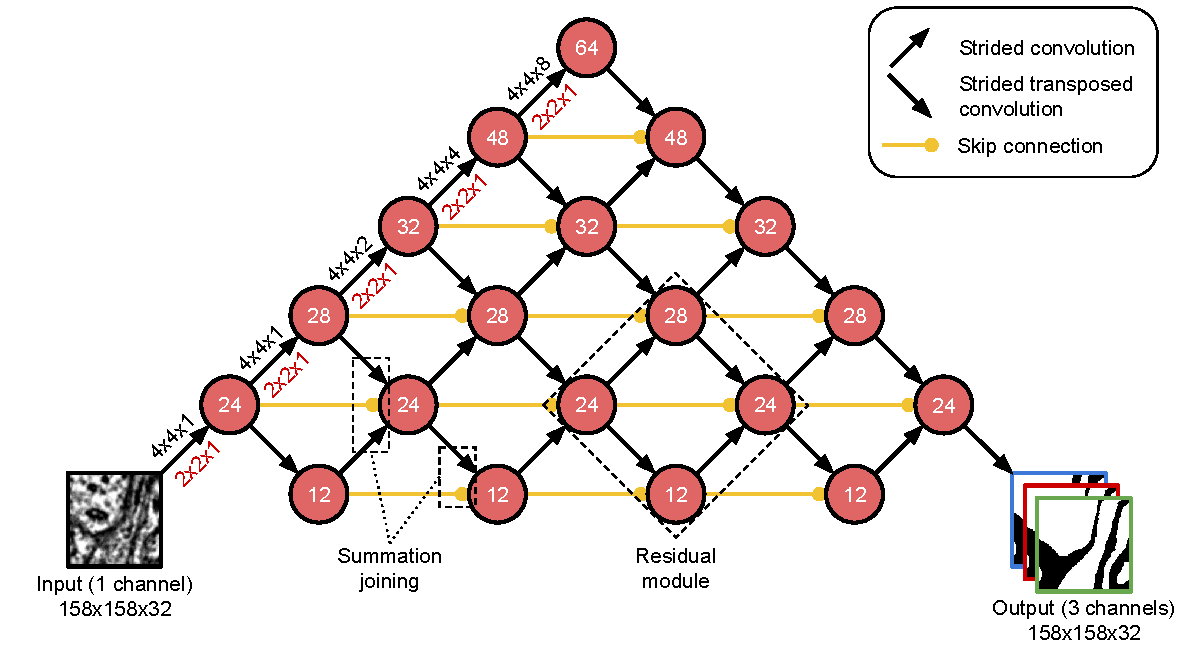
\includegraphics[width=1.0\linewidth]{baseline.pdf}

\caption{Architecture for the baseline neuronal boundary detection. Each node represents a layer and the number inside represents the number of feature maps. The layers closer to the top of the diagram have lower resolution than the layers near the bottom. The diagonal arrows represent strided convolutions, while the horizontal arrows represent skip connections.}
\label{fig:architecture}
\end{figure}

\subsection{Dataset}
A team of tracers produced multiple volumes of gold standard dense reconstruction, in total $20$ volumes of size $512 \times 512 \times 100$. We trained our boundary detector using $19$ volumes and used the last volume for training validation. We then applied the trained boundary detector on a new image volume of size $2048 \times 2048 \times 100$ to obtain a preliminary segmentation, which was then proofread by the tracers to generate a bootstrapped ground truth volume. This volume was used to optimize the parameters for watershed and mean affinity agglomeration. Finally, the optimized segmentation pipeline was applied to generate further bootstrapped ground truth for the error detection and correction.

\subsection{Training procedures}
Our boundary detection networks were implemented based on the Caffe deep
learning framework~\cite{jia2014caffe}. To train our models, we minimized the
binomial cross-entropy loss with class-rebalancing using the Adam
optimizer~\cite{adam}, initialized with $\alpha=0.001$, $\beta_1=0.9$,
$\beta_2=0.999$, and $\epsilon=0.01$. The network weights were initialized
following He et al.~\cite{he2015delving}. The learning rate (or step size
parameter $\alpha$ in the Adam optimizer) was halved when validation loss
plateaud out, up to five times (at $35$K, $175$K, $250$K, $300$K, and $480$K
iterations). We used a single patch of size $158\times158\times32$ (i.e.
minibatch of size 1) to compute gradients at each training iteration. The
training lasted for $800$K iterations until convergence, which took about five
days on a single NVIDIA Titan X Pascal GPU.

\subsection{Inference and postprocessing}
We perform \emph{overlap-blending} inference followed by watershed and mean affinity agglomeration~\cite{kisuk}. We refer the interested readers to~\cite{kisuk} for further details.

%-------------------------------------------------------------------------------
% Section B. Network Architecture
%-------------------------------------------------------------------------------
\section{Network architectures}
\label{appendix:architecture}

\begin{figure}
\centering
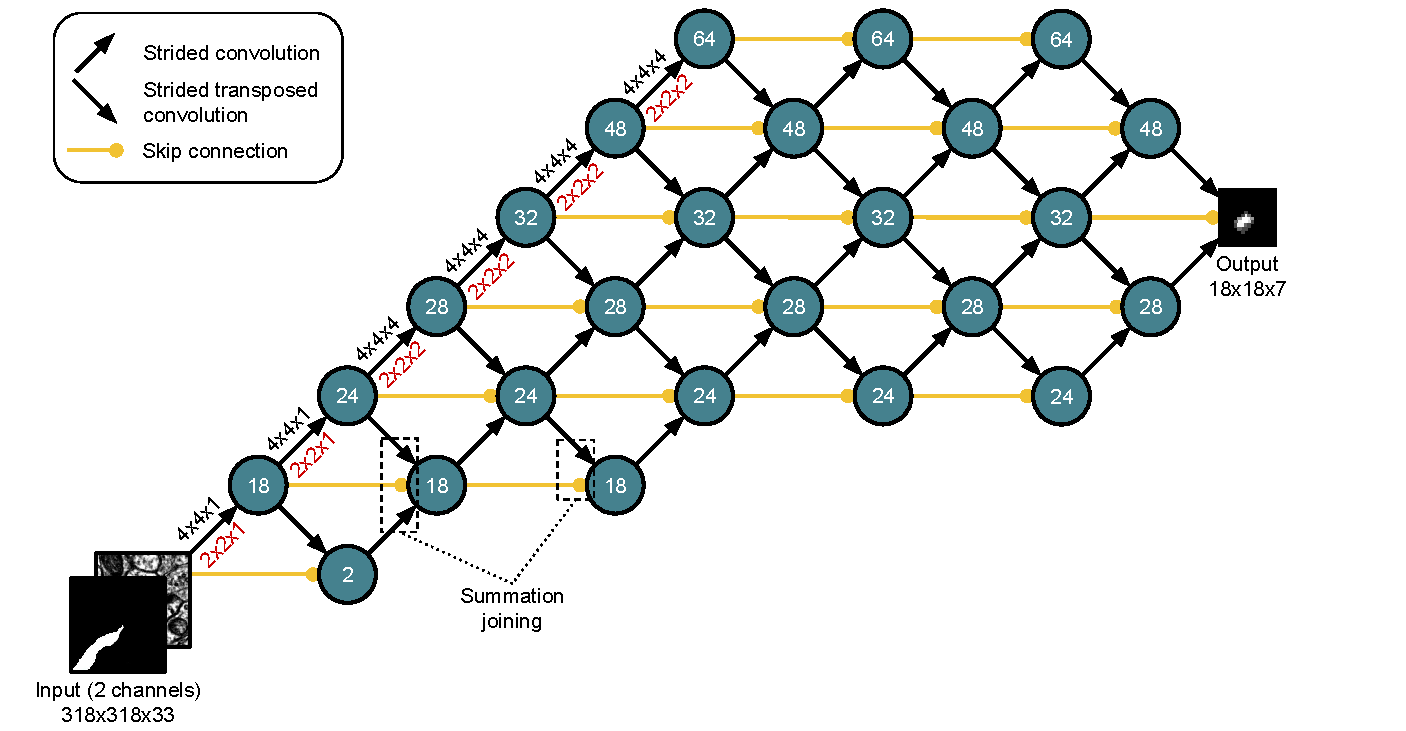
\includegraphics[width=1.0\linewidth]{detector.pdf}
\centering
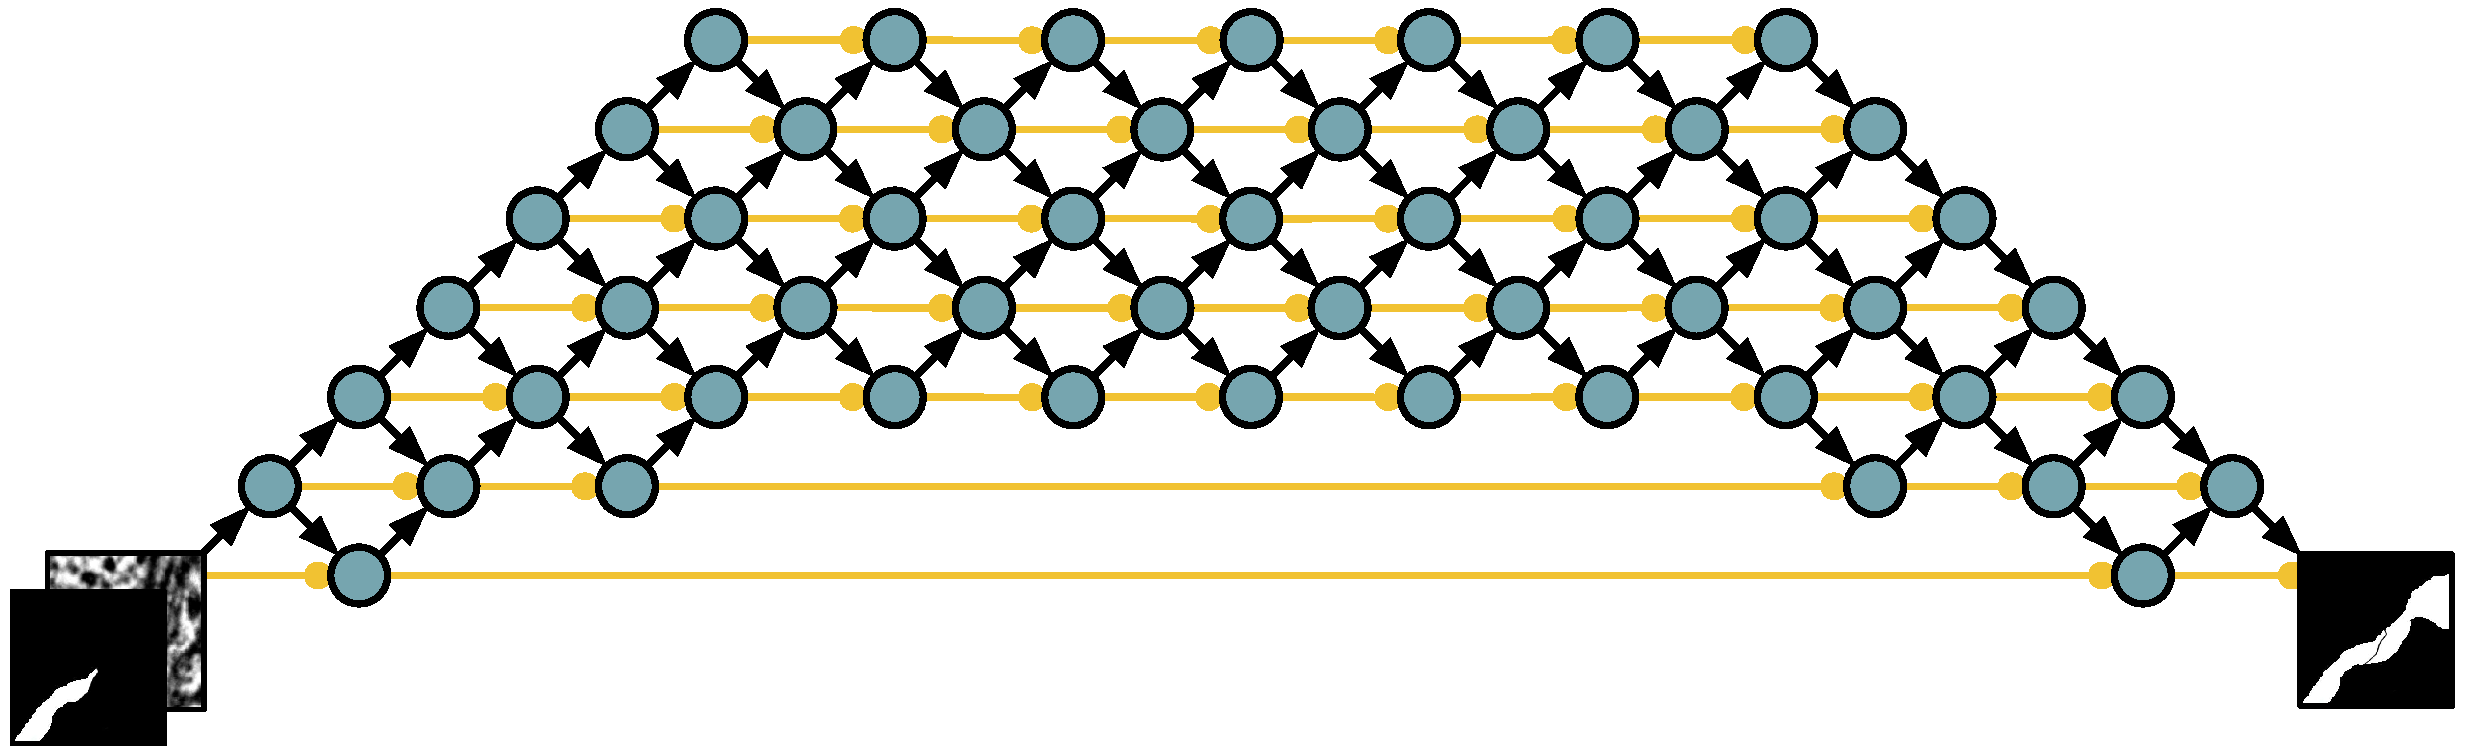
\includegraphics[width=1.0\linewidth]{corrector2.pdf}

\caption{Architectures for the error detection and error correction modules respectively. Each node represents a layer and the number inside represents the number of feature maps. The layers closer to the top of the diagram have lower resolution than the layers near the bottom. We make savings in computation by minimizing the number of high resolution feature maps. The diagonal arrows represent strided convolutions, while the horizontal arrows represent skip connections.}
\label{fig:architecture}
\end{figure}

Due to the anisotropy of the resolution of the images in our dataset, we design our networks so that the first convolutions are exclusively 2D while later convolutions are 3D. The field of view of a unit in the higher layers is therefore roughly cubic.

To limit the number of parameters in our model, we factorize all 3D convolutions into a 2D convolution followed by a 1d convolution in z. We also use weight sharing between some convolutions at the same height.

\section{Per-object VI score}
\label{appendix:vi}
 Recall that the variation of information between two segmentations may be computed as
\begin{align*}
	VI_{split}&=-\frac 1 {\sum_{i,j} r_{ij}} \sum_{i,j} r_{ij} \log(r_{ij}/p_i)\\
	VI_{merge}&=-\frac 1 {\sum_{i,j} r_{ij}} \sum_{i,j} r_{ij} \log(r_{ij}/q_j)\\
	p_i&=\sum_j r_{ij}\\
	q_j&=\sum_i r_{ij}
\end{align*}
where $r_{ij}$ is the number of pixels in common between the $i^{th}$ segment of the ground truth segmentation and the $j^{th}$ segment of the proposed segmentation \cite{vi}.

We define the split and merge scores for ground truth segment $i$ as
\begin{align*}
	VI_{split}(i) &= -\sum_j r_{ij}/p_i \log(r_{ij}/p_i)\\
	VI_{merge}(i) &= -\sum_j r_{ij}/p_i \log(r_{ij}/q_j)
\end{align*}
Both quantities have units of bits. $VI_{split}(i)$ is zero iff ground truth segment $i$ is contained within a segment in the proposed segmentation, while $VI_{merge}(i)$ is zero iff ground truth segment $i$ is the union of one or more segments in the proposed segmentation. The total score $VI_{split}$ or $VI_{merge}$ is a weighted sum of the per-object scores $VI_{split}(i)$, $VI_{merge}(i)$ respectively.


%-------------------------------------------------------------------------------
% Section B. Training Details
%-------------------------------------------------------------------------------
\section{Training details}
The neural networks were implemented in TensorFlow \cite{tensorflow} and trained using 4 TitanX Pascal GPUs with synchronous gradient descent. We used the Adam optimizer \cite{adam}.   Both networks were trained until the loss on a validation set plateaued. The error detection network trained for 700,000 iterations (approximately one week), while the error-correcting network trained for 1,700,000 iterations (approximately three weeks).

\end{appendices}

\bibliography{bib}

\end{document}
